\documentclass[a4paper, 12pt]{article}%тип документа



%отступы
\usepackage[left=1cm,right=1cm,top=1cm,bottom=2cm,bindingoffset=0cm]{geometry}

%%% Работа с русским языком
\usepackage{graphicx}
\usepackage{cmap}                           % поиск в PDF
\usepackage{mathtext} 			 	       % русские буквы в формулах
\usepackage[T2A]{fontenc}               % кодировка
\usepackage[utf8]{inputenc}              % кодировка исходного текста
\usepackage[english,russian]{babel} 
\usepackage{float}
\usepackage{multirow}

\usepackage[export]{adjustbox} % локализация и переносы

\usepackage{subfig}% http://ctan.org/pkg/subfig
\usepackage{booktabs}

\usepackage{wrapfig}


%Матеша
\usepackage{amsmath,amsfonts,amssymb,amsthm,mathtools} % AMS
\usepackage{icomma} % "Умная" запятая

%\mathtoolsset{showonlyrefs=true} % Показывать номера только у тех формул, на которые есть \eqref{} в тексте.

%% Шрифты
\usepackage{euscript}	 % Шрифт Евклид
\usepackage{mathrsfs} % Красивый матшрифт

%% Свои команды
\DeclareMathOperator{\sgn}{\mathop{sgn}}

%% Перенос знаков в формулах (по Львовскому)
\newcommand*{\hm}[1]{#1\nobreak\discretionary{}
	{\hbox{$\mathsurround=0pt #1$}}{}}


%\usepackage{caption}
%\usepackage{subcaption}

\date{15 ноября 2022 г.}
\author{Гаврилин Илья Дмитриевич \\
	Б01-101}
\title{\textbf{Работа 3.3.4 \\ 
		Эффект Холла в полупроводниках}}
\begin{document}
	\maketitle
	\section{Аннотация}
	В данной работе изучили эффект Холла на образце из германия. Замерили ЭДС Холла при различных значениях магнитной индукции, получили значение подвижности носителей тока и их концентрации. Оценили погрешности полученных величин.
	\section{Теоретическая справка}
	Суть эффекта Холла состоит в следующем. Пусть через однородную пластину металла вдоль оси $x$ течет ток $I$ (рис. 1).
	
	\begin{wrapfigure}{l}{0.6\textwidth}
		\vspace{-20pt}
		\begin{center}
			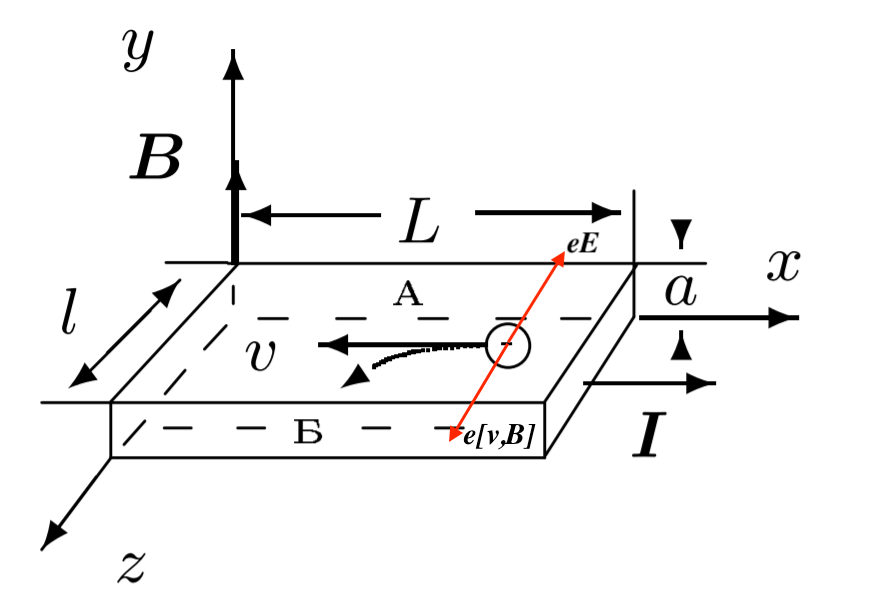
\includegraphics[width=0.7\linewidth]{Holl1.png}
			\label{fig:sdfsafd}
		\end{center}
		\vspace{-20pt}
		\caption{Образец с током в магнитном поле}
	\end{wrapfigure}
	
	Если эту пластину поместить в магнитное поле, направленное по оси y, то между гранями А и Б появляется разность потенциалов. 
	
	В самом деле, на электрон (для простоты рассматриваем один тип носителей), движущийся со средней скоростью $\langle \vec{v} \rangle$ в электромагнитном поле, действует сила Лоренца:
	
	$$\vec{F}_{л} = -e\vec{E}-e \langle \vec{v} \rangle \times \vec{B},$$
	
	где $e$- абсолютный заряд электрона, $\vec{E}$ - напряженность электрического поля, $\vec{B}$ - индукция магнитного поля.
	
	В проекции на ось $z$ получаем
	
	$$ F_{B}=e | \langle {v_{x}} \rangle | B.$$
	
	Под действием этой силы электроны отклоняются к грани Б, заряжая ее отрицательно. На грани А накапливаются нескомпенсированные положительные заряды. Это приводит к возникновению электрического поля $E_{z}$, направленного от А к Б, которое действует на электроны с силой $F_{E}=eE_{z}$. В установившемся режиме $F_{E}=F_{B}$, поэтому накопление электрических зарядов на боковых гранях пластины прекращается. Отсюда
	
	$$ E_{z}=| \langle {v_{x}} \rangle | B.$$
	
	С этим полем связана разность потенциалов $$U_{AБ}=E_{z}l=| \langle {v_{x}} \rangle | Bl.$$
	
	В этом и состоит эффект Холла.
	
	\
	
	Замечая, что сила тока
	
	$$ I=ne| \langle {v_{x}} \rangle |la,$$
	
	найдем ЭДС Холла:
	
	\begin{equation}\label{Rx}
		\mathscr{E}_{X}=U_{AБ}=\dfrac{IB}{nea}=R_{X}\dfrac{IB}{a}
	\end{equation}
	
	Константа $R_{X}=\dfrac{1}{ne}$ называется постоянной Холла.
	
	В полупроводниках, когда вклад в проводимость обусловлен и электронами и дырками, выражение для постоянной Холла имеет более сложный вид:
	
	$$R_{X}=\dfrac{nb^{2}_{e}-pb^{2}_{p}}{e(nb_{e}+pb_{p})^{2}},$$
	
	где $n$ и $p$ - концентрации электронов и дырок, $b_{e}$ $b_{p}$ - их подвижности.
	\section{Ход работы}
	1) Подготовим экспериментальную установку в соответствии с описанием.\\
	2) Изучим характеристики установки: $I_{max} = 2~A$, $a = 1.5\pm0.1~mm$, $L_{3, 5} = 3.0\pm0.1~mm$, $l=1.7\pm0.1~mm$, $SN=75~см^2~вит$, $r_{внш}=5~Ohm$.\\
	\subsection*{Градуировка магнита}
	3) Проведем градуировку оборудования.\\
	\begin{table}[H]
		\centering
		\begin{tabular}{|l|c|c|c|c|c|c|c|c|}
			\hline
			U, В     & 13.2  & 26.8  & 40.4  & 53.6  & 67    & 80.9  & 94.8  & 109   \\ \hline
			I, А     & 0.25  & 0.50  & 0.75  & 1.00  & 1.25  & 1.50  & 1.75  & 2.00  \\ \hline
			$\Phi_1$, mWb & 4.10  & 5.20  & 6.30  & 7.30  & 8.25  & 8.90  & 9.50  & 9.90  \\ \hline
			$\Phi_2$, mWb      & 2.90  & 2.90  & 2.90  & 2.90  & 2.90  & 2.90  & 3.00  & 3.10  \\ \hline
			$\Delta \Phi$, mWb  & 1.20  & 2.30  & 3.40  & 4.40  & 5.35  & 6.00  & 6.50  & 6.80  \\ \hline
			$B$, Тл        & 0.160 & 0.307 & 0.453 & 0.587 & 0.713 & 0.800 & 0.867 & 0.907 \\ \hline
		\end{tabular}
	\caption{Градуировка электромагнита}
	\end{table}
	Рассчитав погрешность получаем: $\Delta B = 0.007~Тл$.\\
	\begin{figure}[H]
		\centering
		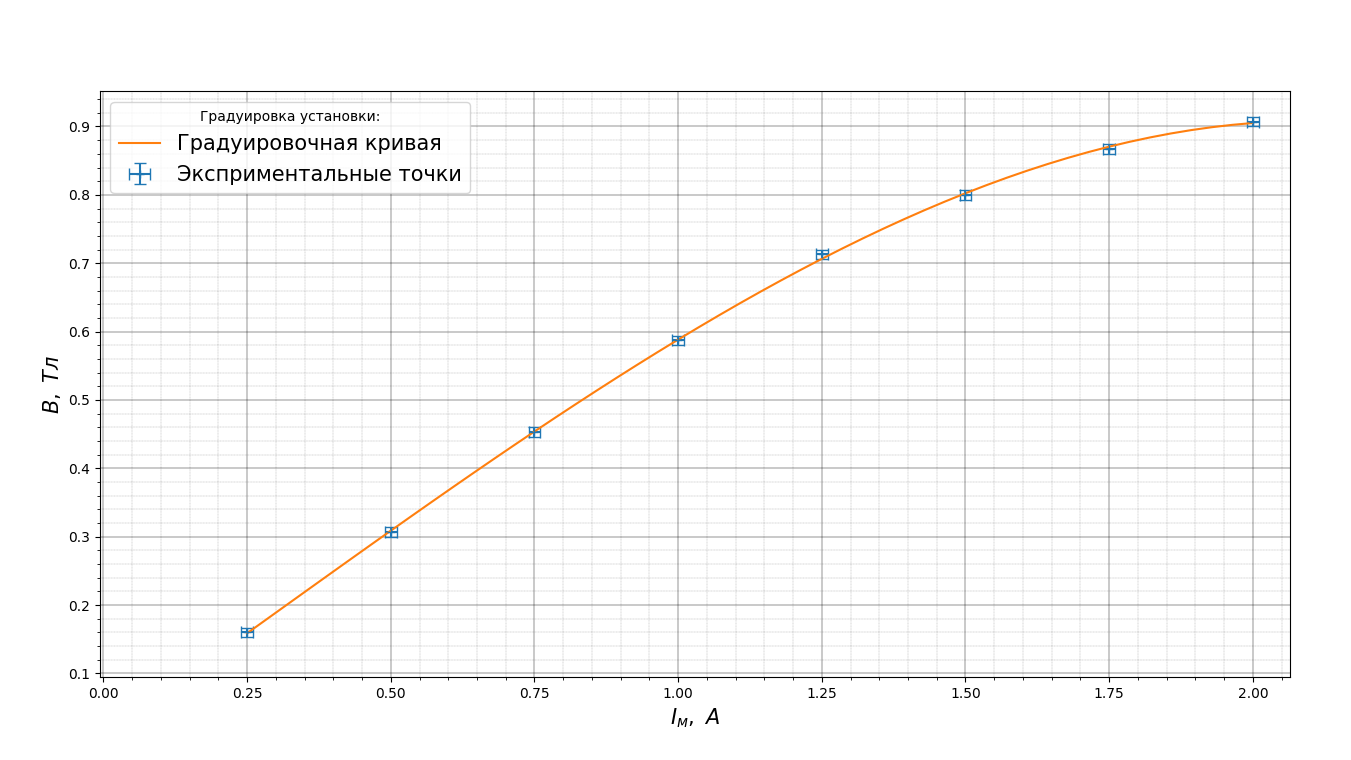
\includegraphics[width=0.8\linewidth]{graduir}
		\caption{Градуировка магнита}
		\label{fig:graduir}
	\end{figure}
	\subsection*{Измерение ЭДС Холла}
	\begin{table}[H]
		\centering
		\begin{tabular}{|c|c|c|c|c|c|c|c|c|c|c|}
			\hline
			\multicolumn{1}{|l|}{}    & B, Тл               & 0.000  & 0.160  & 0.307  & 0.453  & 0.587  & 0.713  & 0.800  & 0.867  & 0.907  \\ \hline
			\multirow{2}{*}{I=0.3 mA}  & U, мВ               & -0.026 & -0.043 & -0.066 & -0.089 & -0.109 & -0.126 & -0.140 & -0.149 & -0.156 \\ \cline{2-11} 
			& $\varepsilon_x$, мВ & 0.000  & -0.017 & -0.040 & -0.063 & -0.083 & -0.100 & -0.114 & -0.123 & -0.130 \\ \hline
			\multirow{2}{*}{I=0.4 mA}  & U, мВ               & -0.028 & -0.058 & -0.090 & -0.119 & -0.148 & -0.172 & -0.189 & -0.201 & -0.210 \\ \cline{2-11} 
			& $\varepsilon_x$, мВ & 0.000  & -0.030 & -0.062 & -0.091 & -0.120 & -0.144 & -0.161 & -0.173 & -0.182 \\ \hline
			\multirow{2}{*}{I=0.5 mA}  & U, мВ               & -0.036 & -0.073 & -0.112 & -0.150 & -0.183 & -0.214 & -0.236 & -0.251 & -0.263 \\ \cline{2-11} 
			& $\varepsilon_x$, мВ & 0.000  & -0.037 & -0.076 & -0.114 & -0.147 & -0.178 & -0.200 & -0.215 & -0.227 \\ \hline
			\multirow{2}{*}{I=0.6 mA}  & U, мВ               & -0.043 & -0.087 & -0.135 & -0.179 & -0.220 & -0.257 & -0.283 & -0.301 & -0.316 \\ \cline{2-11} 
			& $\varepsilon_x$, мВ & 0.000  & -0.044 & -0.092 & -0.136 & -0.177 & -0.214 & -0.240 & -0.258 & -0.273 \\ \hline
			\multirow{2}{*}{I=0.7 mA}  & U, мВ               & -0.050 & -0.102 & -0.158 & -0.209 & -0.257 & -0.300 & -0.330 & -0.351 & -0.367 \\ \cline{2-11} 
			& $\varepsilon_x$, мВ & 0.000  & -0.052 & -0.108 & -0.159 & -0.207 & -0.250 & -0.280 & -0.301 & -0.317 \\ \hline
			\multirow{2}{*}{I=0.8 mA}  & U, мВ               & -0.057 & -0.118 & -0.179 & -0.240 & -0.293 & -0.342 & -0.376 & -0.401 & -0.420 \\ \cline{2-11} 
			& $\varepsilon_x$, мВ & 0.000  & -0.061 & -0.122 & -0.183 & -0.236 & -0.285 & -0.319 & -0.344 & -0.363 \\ \hline
			\multirow{2}{*}{I=0.9 mA}  & U, мВ               & -0.064 & -0.130 & -0.201 & -0.270 & -0.331 & -0.383 & -0.425 & -0.451 & -0.473 \\ \cline{2-11} 
			& $\varepsilon_x$, мВ & 0.000  & -0.066 & -0.137 & -0.206 & -0.267 & -0.319 & -0.361 & -0.387 & -0.409 \\ \hline
			\multirow{2}{*}{I=1 mA} & U, мВ               & -0.061 & 0.013  & 0.089  & 0.160  & 0.225  & 0.280  & 0.321  & 0.350  & 0.371  \\ \cline{2-11} 
			& $\varepsilon_x$, мВ & 0.000  & 0.074  & 0.150  & 0.221  & 0.286  & 0.341  & 0.382  & 0.411  & 0.432  \\ \hline
		\end{tabular}
		\caption{Измерение ЭДС Холла}
	\end{table}
	$\varepsilon_x$ подсчитали как разность с показанием напряжения при выключенном магните.\\
	\subsection*{Поиск коэффициентов наклона}
	По полученным данным построим графики зависимости $\varepsilon_x=f(B)$, аппроксимируем экспериментальные точки прямой, получим угловые коэффициенты наклона.\\
	\begin{figure}[H]
		\centering
		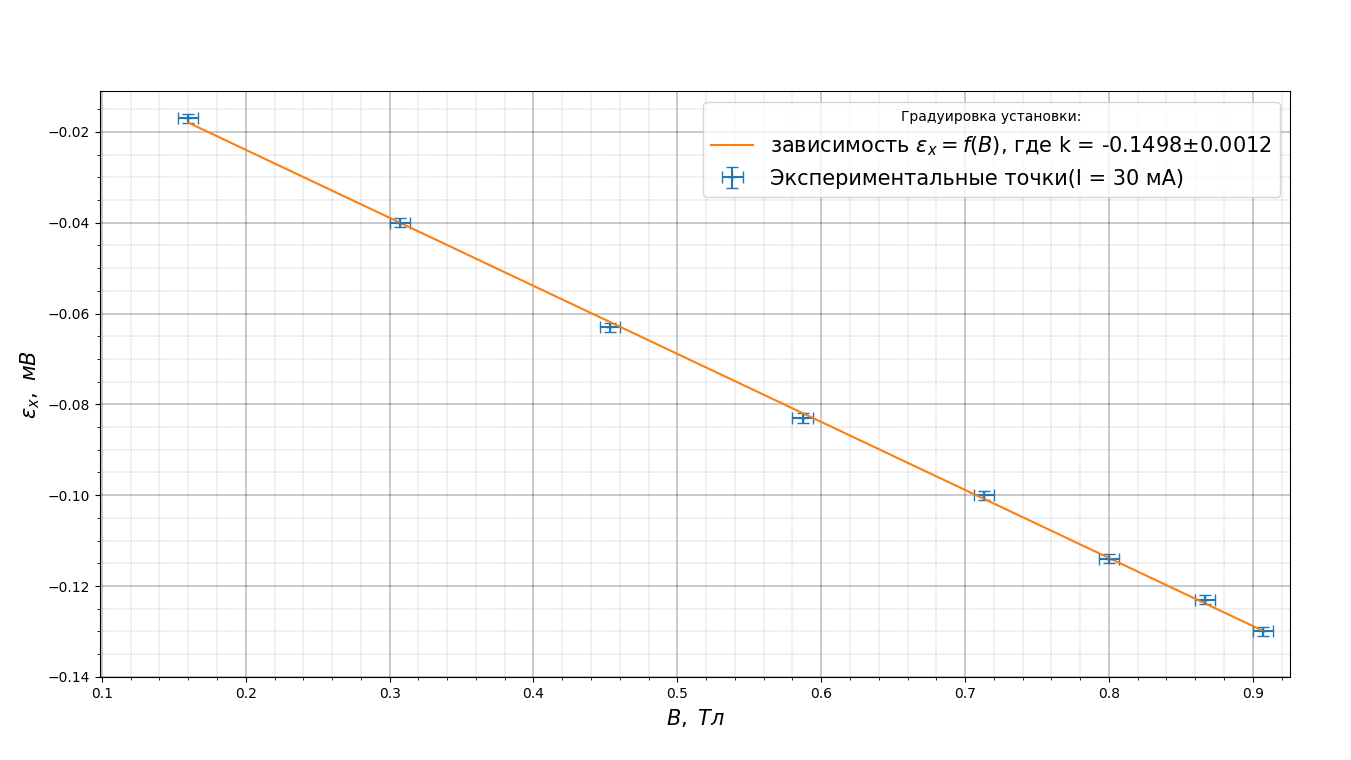
\includegraphics[width=0.8\linewidth]{30}
		\caption{Зависимость ЭДС Холла от B}
		\label{fig:30}
	\end{figure}
	\begin{figure}[H]
		\centering
		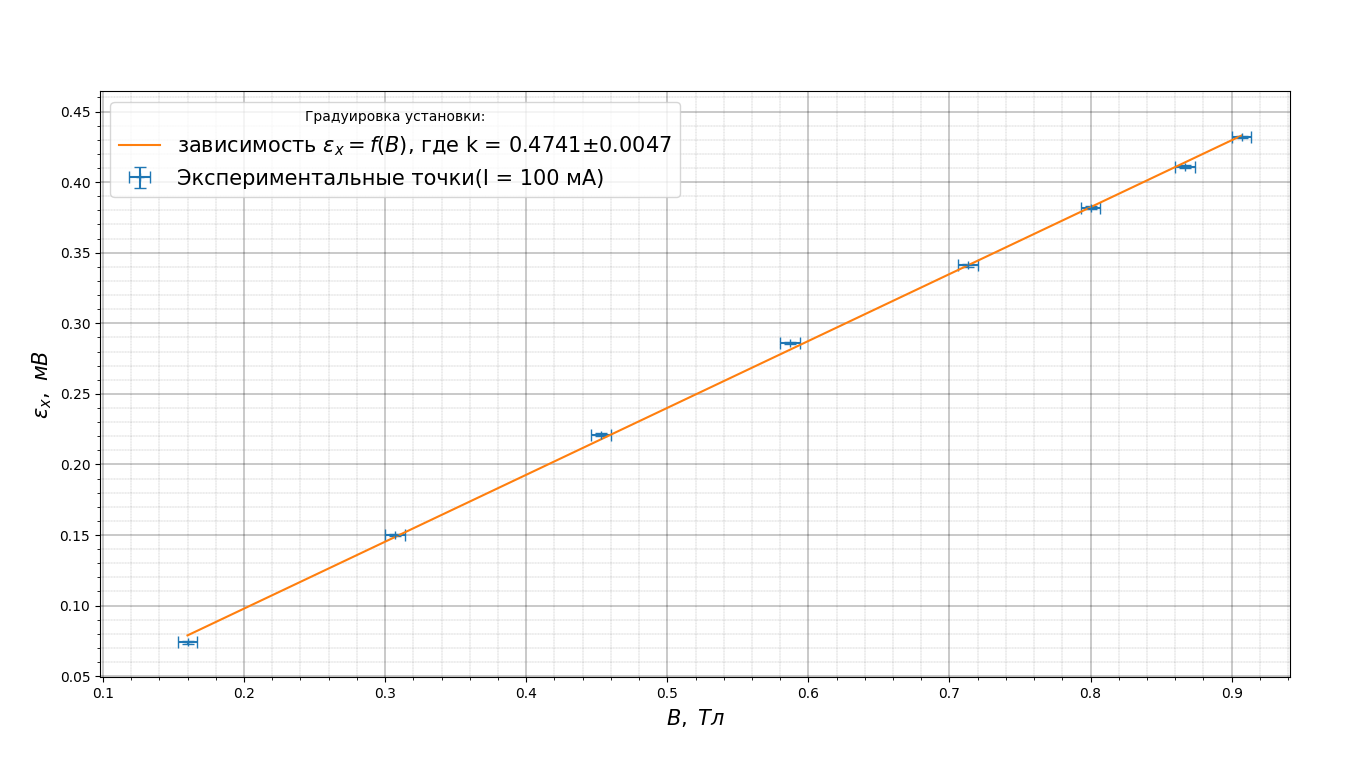
\includegraphics[width=0.8\linewidth]{100}
		\caption{Зависимость ЭДС Холла от B, при реверсивной полярности}
		\label{fig:100}
	\end{figure}
	\begin{figure}[H]
		\centering
		\subfloat[$I=0.4 мA$ ]{{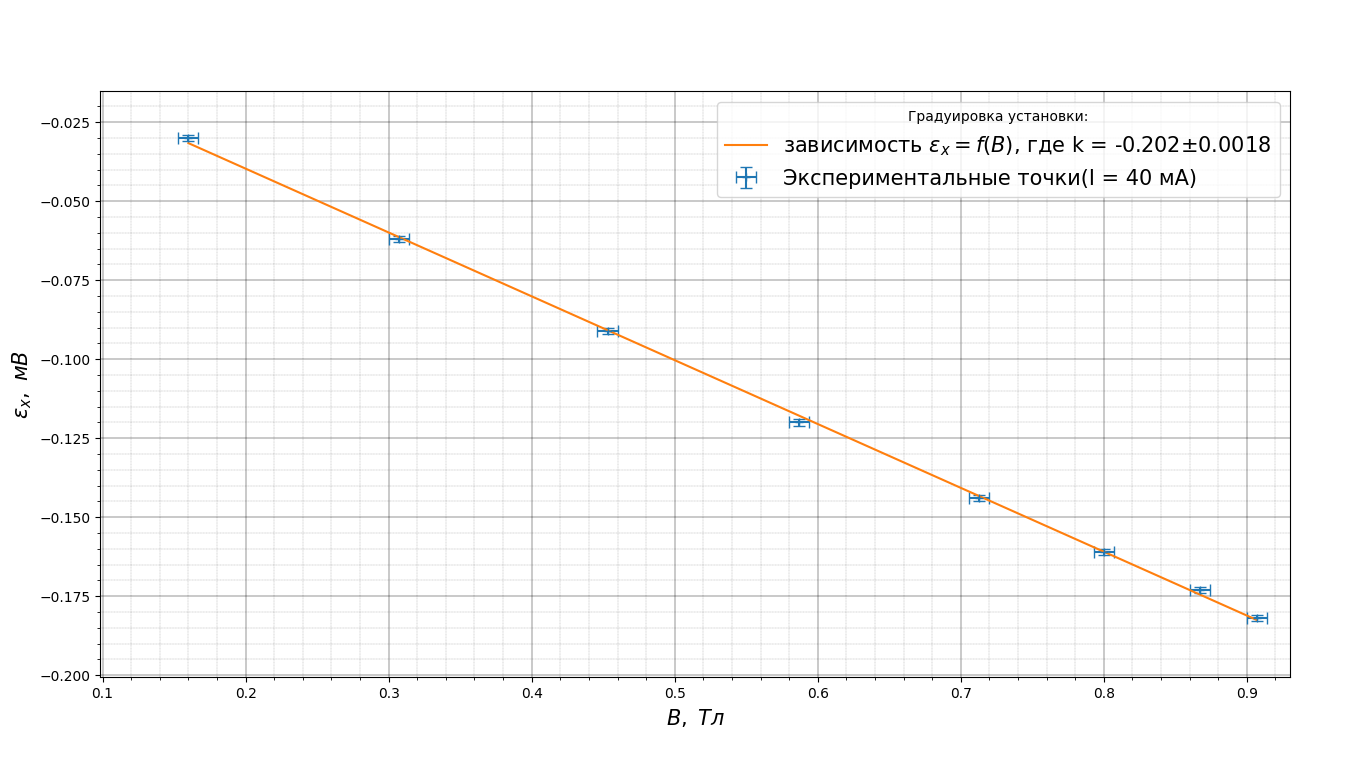
\includegraphics[width=0.478\textwidth]{40}}}
		\qquad
		\subfloat[$I=0.5 мA$ ]{{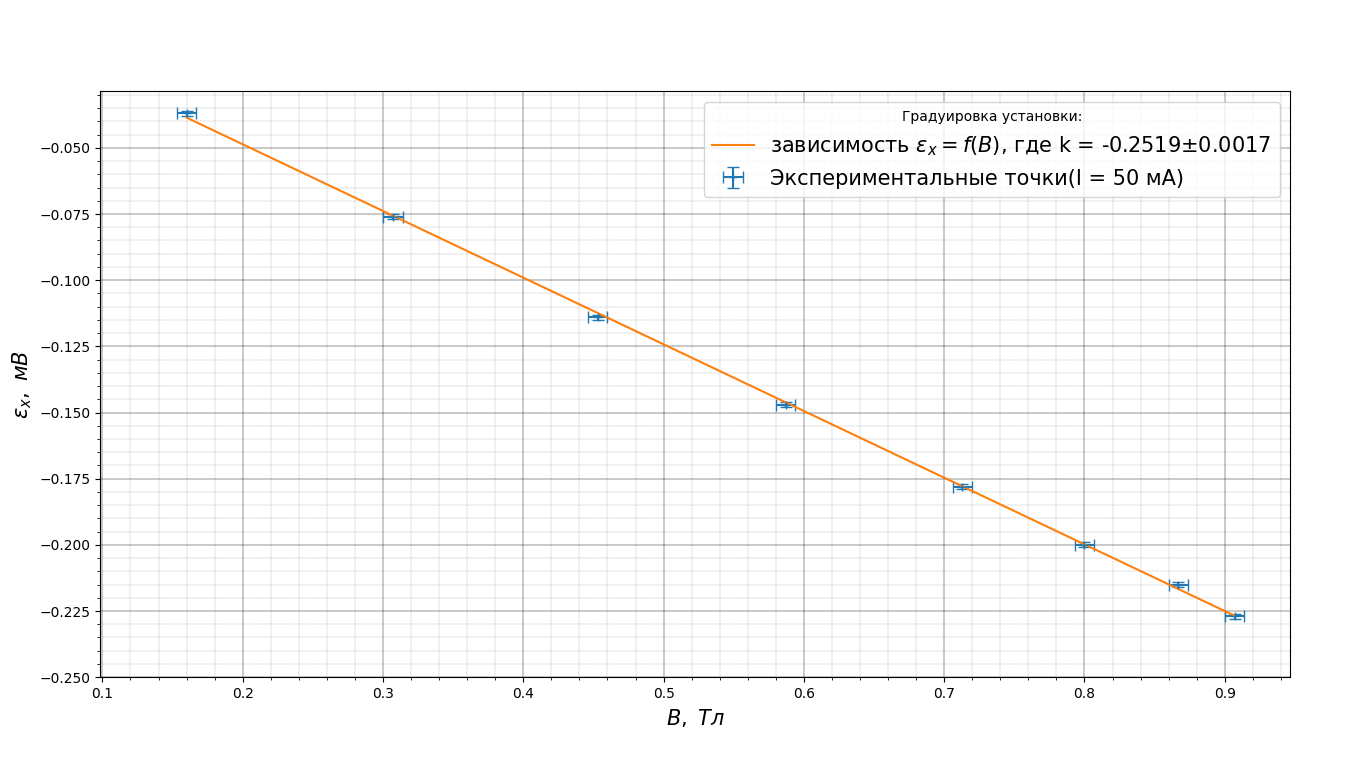
\includegraphics[width=0.478\textwidth]{50}}}\\
		\subfloat[$I=0.6 мA$]{{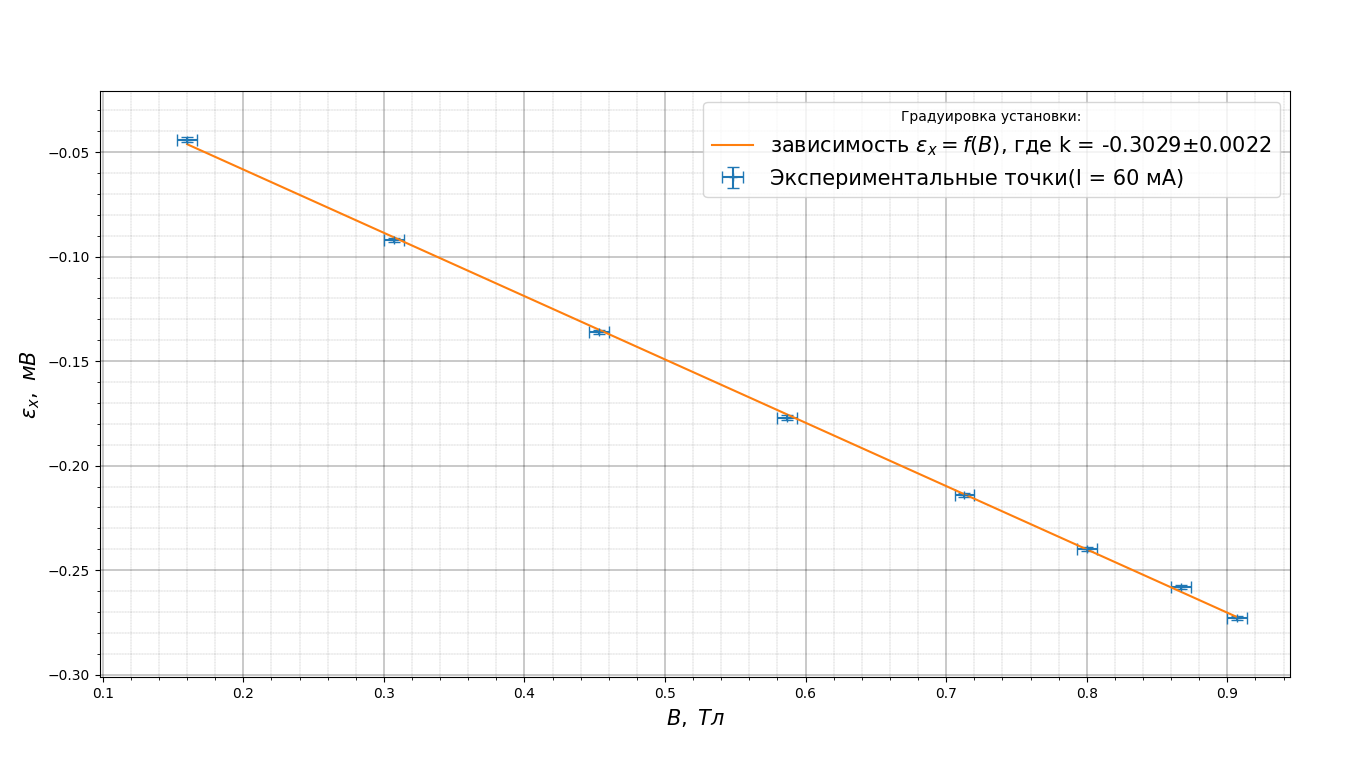
\includegraphics[width=0.478\textwidth]{60}}}
		\qquad
		\subfloat[$I=0.7 мA$]{{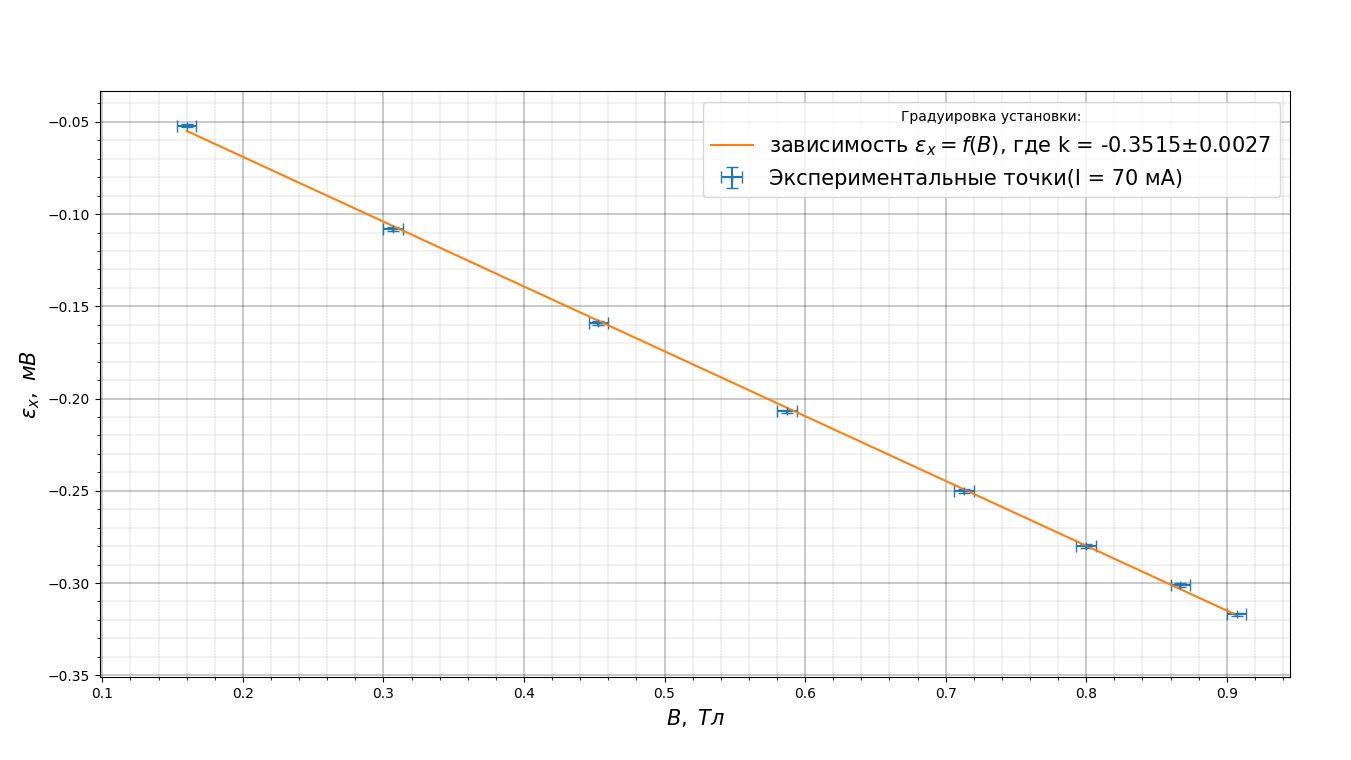
\includegraphics[width=0.478\textwidth]{70}}}\\
			\subfloat[$I=0.8 мA$]{{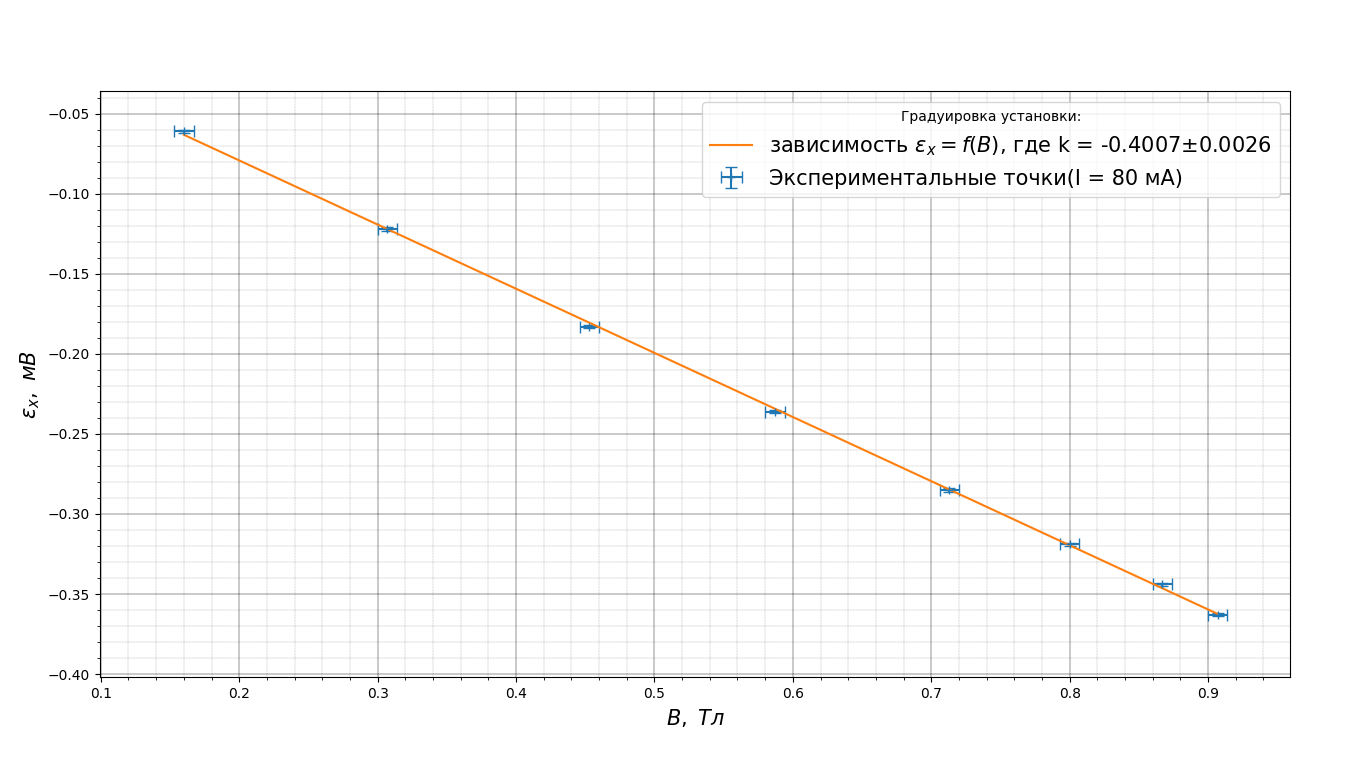
\includegraphics[width=0.478\textwidth]{80}}}
		\qquad
		\subfloat[$I=0.9 мA$]{{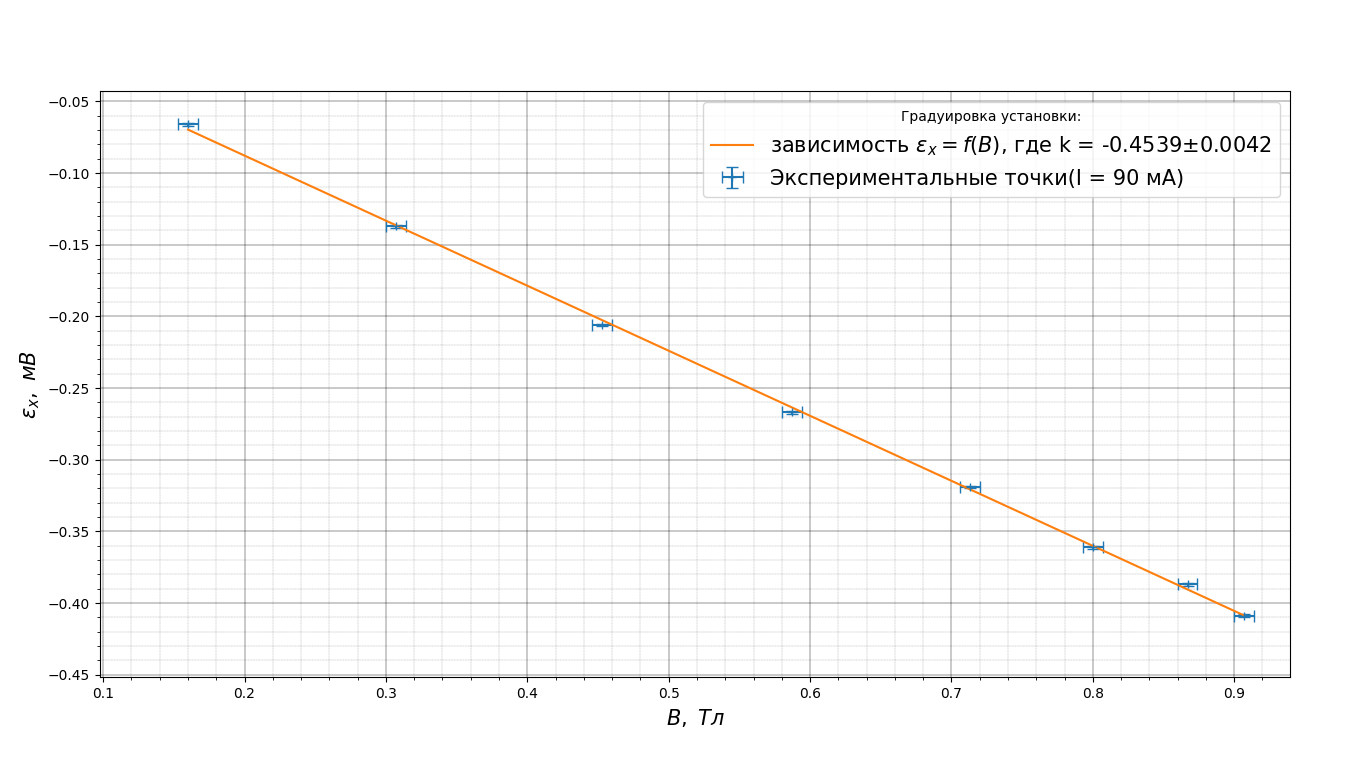
\includegraphics[width=0.478\textwidth]{90}}}
		\caption{Зависимость ЭДС Холла от B}
	\end{figure}
	\subsection*{Зависимость коэффициента наклона от тока}
	\begin{table}[H]
		\centering
		\begin{tabular}{|l|l|l|l|l|l|l|l|l|}
			\hline
			$I,  мA$ & 0.3     & \multicolumn{1}{c|}{0.4} & \multicolumn{1}{c|}{0.5} & \multicolumn{1}{c|}{0.6} & \multicolumn{1}{c|}{0.7} & \multicolumn{1}{c|}{0.8} & \multicolumn{1}{c|}{0.9} & \multicolumn{1}{c|}{1} \\ \hline
			$k\cdot10^{-3}$, В/Тл  & 0.1498 & 0.202                   & 0.2519                  & 0.3029                  & 0.3515                  & 0.4007                  & 0.4539                  & 0.4741                   \\ \hline
				$\Delta k\cdot10^{-3}$, В/Тл      & 0.0012 & 0.0018                  & 0.0017                  & 0.022                   & 0.0027                  & 0.0026                  & 0.0022                  & 0.0047                   \\ \hline
		\end{tabular}
		\caption{Зависимость коэффициента наклона от тока текущего через образец}
	\end{table}
	\begin{figure}[H]
		\centering
		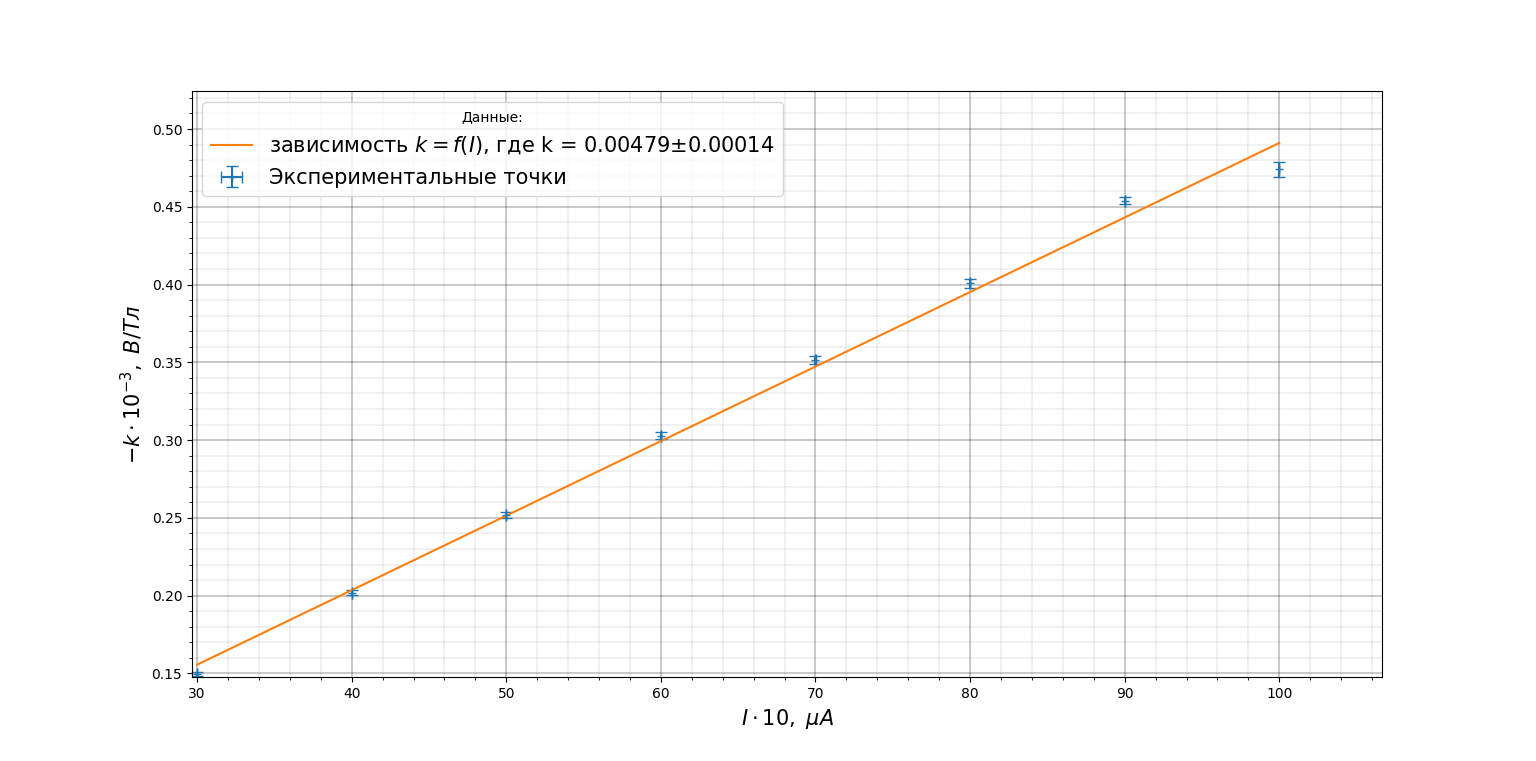
\includegraphics[width=0.8\linewidth]{k}
		\caption{Зависимость k от тока протекающего через образец}
		\label{fig:k}
	\end{figure}
	Получили $k = 0.479 \pm 0.014$ В/Тл * А. \\
	Тогда: $R_x=(7.2\pm 0.4)*10^{-4} ~м^3/Кл$, тогда $n=(868\pm1)\cdot 10^{19}~м^3$.\\
	$\sigma = (692 \pm 1.2) ~(Ом\cdot м)^{-1}$\\
	$b = \frac{\sigma}{en} = (5000 \pm 50) \frac{см^2}{В\cdot c}$
	\section{Выводы}
	1) Тип носителей заряда - дырочный.\\
	3) Нашли Все требуемые характеристики полупроводника (см п.3 Зависимость коэффициента наклона от тока).\\
	
	
	
	
\end{document}